
% ===================================================================
% FILE: Lezione17.tex
% ===================================================================

% --- Definizioni Locali (Compatibilità) ---

% (Rimosso codebox locale)

% Adattamento ambiente 'proposition' usando 'concept' (stile Bibbia)
\newenvironment{proposition}[1][Proposizione]
  {\begin{concept}{#1}}
  {\end{concept}}

\part{Lezione 17: Alberi Binari: Bilanciamento e Proprietà Avanzate}

\section{Schema Generale di Ricorsione su Alberi}

Quando si affrontano problemi su alberi binari che richiedono di calcolare una proprietà o un valore basato sulla struttura dell'albero, si utilizza spesso uno schema ricorsivo standard basato sulla proprietà di \textbf{decomponibilità} del problema.

\begin{concept}{Schema di Risoluzione Decomponibile}
L'algoritmo segue questi passi fondamentali:
\begin{enumerate}
    \item \textbf{Caso Base:} Si gestisce l'albero vuoto (o foglia), restituendo un valore neutro o specifico per la chiusura della ricorrenza (es. 0, null, true).
    \item \textbf{Passo Induttivo (Divide):} Si effettuano le chiamate ricorsive sui sottoalberi sinistro (\texttt{u.left}) e destro (\texttt{u.right}).
    \item \textbf{Combinazione (Conquer):} Si combinano i risultati ottenuti dai sottoalberi con le informazioni del nodo corrente (\texttt{u}) per ottenere il risultato finale.
    \item \textbf{Restituzione:} Si restituisce l'esito al chiamante (caso generale).
\end{enumerate}
\end{concept}

\subsection{Implementazione Generica e Complessità}

Di seguito lo pseudocodice generico per una funzione \texttt{DECOMP(u)} che opera su un nodo \texttt{u}.

\begin{codebox}{Pseudocodice: DECOMP(u)}
\begin{verbatim}
Funzione DECOMP(u)
    // 1. Caso Base
    IF (u == NULL) THEN 
        RETURN ValoreBase; 
    
    // 2. Passo Induttivo
    RisSx = DECOMP(u.left);  // Ricorsione a sinistra
    RisDx = DECOMP(u.right); // Ricorsione a destra
    
    // 3. Combinazione
    RETURN RICOMBINA(RisSx, RisDx, u.info);
\end{verbatim}
\end{codebox}

\begin{explanation}{Analisi dello Schema Ricorsivo}
Questo "template" è universale per problemi decomponibili:
\begin{itemize}
    \item \textbf{Discesa (Pre-order)}: Si scende fino alle foglie (null).
    \item \textbf{Risalita (Post-order)}: I risultati parziali (\texttt{RisSx}, \texttt{RisDx}) tornano dai figli e vengono combinati nel nodo corrente.
\end{itemize}
\end{explanation}

\begin{center}
\begin{tikzpicture}[
    node/.style={circle, draw, minimum size=0.8cm},
    arrow/.style={->, thick, blue}
    ]
    \node[node] (u) {u};
    \node[node, below left=of u] (l) {sx};
    \node[node, below right=of u] (r) {dx};
    
    \draw[->] (u) -- (l) node[midway, left, font=\tiny] {1. Call};
    \draw[->] (u) -- (r) node[midway, right, font=\tiny] {2. Call};
    \draw[dashed, ->, red] (l) to[bend left] node[midway, left, font=\tiny] {3. Return} (u);
    \draw[dashed, ->, red] (r) to[bend right] node[midway, right, font=\tiny] {4. Return} (u);
    
    \node[right=of u] {Combine (u.info + sx + dx)};
\end{tikzpicture}
\end{center}

\paragraph{Complessità Computazionale.}
Poiché l'algoritmo visita ogni nodo esattamente una volta (come una visita post-order), la complessità temporale è lineare rispetto al numero di nodi $n$:
$$ T(n) = \Theta(n) $$

---

\section{Alberi Binari Completamente Bilanciati (ABCB)}

Un concetto fondamentale è la distinzione tra un albero completo e uno completamente bilanciato.

\begin{concept}{Definizioni Tassonomiche}
\begin{itemize}
    \item \textbf{Albero Binario Completo:} Un albero binario è \textit{completo} se ogni nodo ha esattamente 0 o 2 figli (nessun nodo ha grado 1).
    \item \textbf{Albero Binario Completamente Bilanciato (ABCB):} È un albero binario che è \textbf{sia completo}, sia ha tutte le \textbf{foglie allo stesso livello}.
\end{itemize}
\end{concept}

\subsection{Proprietà Matematiche degli ABCB}
Dato un ABCB di altezza $h$ (dove l'altezza è il numero di archi dalla radice alla foglia più profonda, oppure definita in base ai nodi come $h_{nodi}$), valgono le seguenti relazioni notevoli:

\begin{itemize}
    \item \textbf{Numero di foglie:} $2^h$.
    \item \textbf{Numero di nodi interni:} $2^h - 1$.
    \item \textbf{Numero totale di nodi ($n$):} Somma di foglie e interni:
    $$ n = 2^h + (2^h - 1) = 2^{h+1} - 1 $$
    \item \textbf{Relazione Altezza-Nodi:} Invertendo la formula:
    $$ n + 1 = 2^{h+1} \implies \log_2(n+1) = h + 1 \implies h = \log_2(n+1) - 1 $$
    Pertanto, l'altezza è logaritmica: $h(n) = \Theta(\log n)$.
\end{itemize}

\subsection{Algoritmo di Verifica ABCB}
Vogliamo scrivere un algoritmo che restituisca \texttt{TRUE} se un albero è ABCB, \texttt{FALSE} altrimenti.

\subsubsection{Approccio 1: Naive (Inefficiente)}
Un primo approccio controlla ricorsivamente se i sottoalberi sono ABCB e se hanno la stessa altezza.
$$ \text{Check}(u) = \text{ABCB}(u.left) \land \text{ABCB}(u.right) \land (H(u.left) == H(u.right)) $$
Questo approccio è inefficiente perché ricalcola l'altezza $H(u)$ ripetutamente per ogni nodo.

\subsubsection{Approccio 2: Ottimizzato (Lineare)}
Per ottenere una complessità $\Theta(n)$, dobbiamo calcolare il bilanciamento e l'altezza in un'unica visita (bottom-up). La funzione restituisce una coppia di valori \texttt{<bool bilanciato, int altezza>}.

\begin{codebox}{Algoritmo: ABCB2(u) $\rightarrow <bool, int>$}
\begin{verbatim}
ABCB2(u):
    // Caso Base: albero vuoto è bilanciato, altezza -1
    IF (u == NULL) THEN 
        RETURN <TRUE, -1>;

    // Chiamate Ricorsive
    <bil_s, alt_s> = ABCB2(u.left);
    <bil_d, alt_d> = ABCB2(u.right);

    // Logica di Combinazione:
    // 1. Sottoalberi devono essere bilanciati (bil_s && bil_d)
    // 2. Altezze devono essere uguali (alt_s == alt_d)
    is_balanced = bil_s AND bil_d AND (alt_s == alt_d);
    
    // Calcolo nuova altezza corrente
    current_height = 1 + max(alt_s, alt_d);

    RETURN <is_balanced, current_height>;
\end{verbatim}
\end{codebox}

\begin{explanation}{Strategia Bottom-Up $O(n)$}
Invece di ricalcolare l'altezza separatamente ($O(n^2)$), la funzione restituisce \textbf{due valori}:
1.  Il booleano di bilanciamento (AND logico dei figli).
2.  L'altezza corrente (aggiornata in risalita).
Questo permette di visitare ogni nodo una sola volta.
\end{explanation}

\textbf{Complessità:} Lineare, $\Theta(n)$, poiché esegue un attraversamento post-order costante per nodo.

---

\section{Nodi Cardine}

Un problema algoritmico interessante riguarda l'identificazione di nodi che soddisfano una specifica proprietà geometrica all'interno dell'albero.

\begin{concept}{Definizione: Nodo Cardine}
Un nodo $u$ di un albero binario si dice \textbf{CARDINE} se e solo se la sua profondità ($P_u$) è uguale alla sua altezza ($h_u$).
$$ u \text{ è Cardine} \iff P_u = h_u $$
\end{concept}
\textit{Nota:} $P_u$ è la distanza dalla radice, $h_u$ è la distanza dalla foglia più profonda nel suo sottoalbero.

\subsection{Strategia Risolutiva}
Per verificare questa condizione in modo efficiente ($\Theta(n)$), dobbiamo:
\begin{enumerate}
    \item Passare la profondità $p$ \textbf{scendendo} nell'albero (parametro in input).
    \item Calcolare l'altezza \textbf{risalendo} dall'albero (valore di ritorno).
    \item Verificare la condizione $p == altezza$ nel post-order.
\end{enumerate}

\begin{codebox}{Algoritmo: CARDINE(u, p)}
\begin{verbatim}
// Input: u (nodo corrente), p (profondità corrente, inizialmente 0)
// Output: altezza del sottoalbero radicato in u

INT CARDINE(Node u, int p)
    // 1. Caso Base
    IF (u == NULL) THEN 
        RETURN -1;

    // 2. Discesa ricorsiva (aumento profondità)
    int alt_s = CARDINE(u.left, p + 1);
    int alt_d = CARDINE(u.right, p + 1);

    // 3. Calcolo Altezza (fase di risalita)
    int \texttt{my\_alt} = max(alt_s, alt_d) + 1;

    // 4. Verifica proprietà Cardine
    IF (p == \texttt{my\_alt}) THEN 
        PRINT(u.key);

    RETURN \texttt{my\_alt};
\end{verbatim}
\end{codebox}

\begin{explanation}{Doppio Flusso Informativo}
Qui combiniamo due direzioni:
\begin{itemize}
    \item \textbf{Input (Top-down)}: La profondità \texttt{p} viene passata dal padre al figlio incrementandola.
    \item \textbf{Output (Bottom-up)}: L'altezza \texttt{\texttt{my\_alt}} viene calcolata dalle foglie risalendo.
    \item La verifica \texttt{p == \texttt{my\_alt}} avviene nel momento di incontro (post-order).
\end{itemize}
\end{explanation}

\subsection{Esempio di Traccia (Trace)}
Consideriamo l'albero tracciato nei sorgenti.
\begin{center}
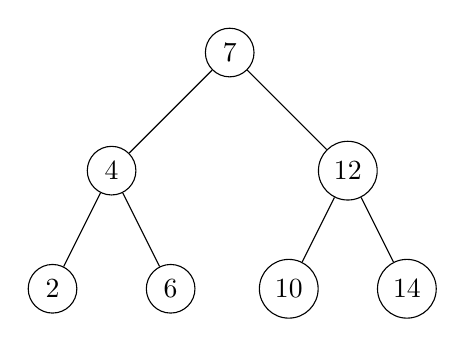
\begin{tikzpicture}[level distance=1.5cm,
  level 1/.style={sibling distance=3cm},
  level 2/.style={sibling distance=1.5cm}]
  \node[circle, draw] {7}
    child {node[circle, draw] {4}
      child {node[circle, draw] {2}}
      child {node[circle, draw] {6}}
    }
    child {node[circle, draw] {12}
      child {node[circle, draw] {10}}
      child {node[circle, draw] {14}}
    };
\end{tikzpicture}
\end{center}

Analisi per alcuni nodi (supponendo struttura bilanciata dall'esempio):
\begin{itemize}
    \item \textbf{Nodo 7 (Radice):} Profondità $P=0$, Altezza $h=2$. ($0 \neq 2$) $\rightarrow$ No.
    \item \textbf{Nodo 4:} Profondità $P=1$, Altezza $h=1$. ($1 = 1$) $\rightarrow$ \textbf{CARDINE}.
    \item \textbf{Nodo 12:} Profondità $P=1$, Altezza $h=1$. ($1 = 1$) $\rightarrow$ \textbf{CARDINE}.
    \item \textbf{Foglie (2, 6, 10, 14):} Profondità $P=2$, Altezza $h=0$. ($2 \neq 0$) $\rightarrow$ No.
\end{itemize}

---

\section{Esercizi per Casa}

\subsection{Nodi Centrali}
\textbf{Problema:} Progettare un algoritmo che, dato un Albero Binario, stampi le chiavi dei suoi \textbf{Nodi Centrali}.

\begin{concept}{Definizione: Nodo Centrale}
Un nodo $u$ è detto \textbf{CENTRALE} se la dimensione del sottoalbero di cui è radice (numero di nodi) è uguale alla somma delle chiavi dei nodi che appartengono al percorso dalla radice al nodo stesso.
$$ Size(u) = \sum_{v \in \text{Path}(root \to u)} v.key $$
\end{concept}

\paragraph{Suggerimento per la soluzione:}
L'algoritmo deve combinare due flussi di informazioni, similmente all'esercizio sui Nodi Cardine:
1. \textbf{Top-down (Parametro):} La somma delle chiavi dalla radice al padre + chiave corrente.
2. \textbf{Bottom-up (Return):} La dimensione del sottoalbero (1 + size(sx) + size(dx)).
3. \textbf{Verifica:} Nel passo di post-order, confrontare i due valori.

\begin{codebox}{Abbozzo Soluzione: CENTRALE(u, somma\_cammino)}
\begin{verbatim}
CENTRALE(u, somma_corrente):
    IF u == NULL RETURN 0
    
    nuova_somma = somma_corrente + u.key
    
    size_sx = CENTRALE(u.left, nuova_somma)
    size_dx = CENTRALE(u.right, nuova_somma)
    
    my_size = 1 + size_sx + size_dx
    
    IF (my_size == nuova_somma) PRINT u.key
    
    RETURN my_size
\end{verbatim}
\end{codebox}

\begin{explanation}{Logica Nodi Centrali}
Simile ai nodi cardine, ma accumulando la somma delle chiavi:
\begin{itemize}
    \item \texttt{somma\_corrente} scende (Pre-order).
    \item \texttt{my\_size} (dimensione sottoalbero) risale (Post-order).
\end{itemize}
\end{explanation}
